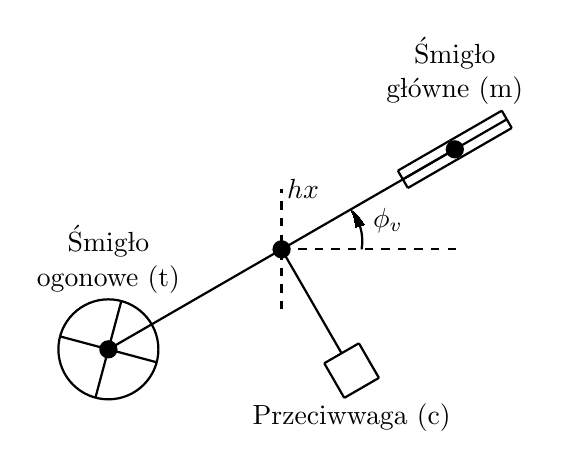
\begin{tikzpicture}[scale=2.54]
% dpic version 2015.10.28 option -g for TikZ and PGF 1.01
\ifx\dpiclw\undefined\newdimen\dpiclw\fi
\global\def\dpicdraw{\draw[line width=\dpiclw]}
\global\def\dpicstop{;}
\dpiclw=0.8bp
\dpicdraw (0.25,0) circle (0.098425in)\dpicstop
\dpicdraw (0.314714,0.241479)
 --(0.185264,-0.241473)\dpicstop
\dpicdraw (0.491482,-0.064703)
 --(0.008512,0.064681)\dpicstop
\dpicdraw[fill=black](0.25,0) circle (0.015748in)\dpicstop
\dpicdraw (0.25,0)
 --(1.116033,0.499987)\dpicstop
\dpicdraw[fill=black](1.116033,0.499987) circle (0.015748in)\dpicstop
\dpicdraw (1.116033,0.499987)
 --(1.982066,0.999973)\dpicstop
\dpicdraw (1.722266,0.849975)
 --(1.747268,0.806674)\dpicstop
\dpicdraw (1.747268,0.806674)
 --(2.007077,0.95667)\dpicstop
\dpicdraw (2.007077,0.95667)
 --(2.266887,1.106666)\dpicstop
\dpicdraw (2.266887,1.106666)
 --(2.24189,1.149969)\dpicstop
\dpicdraw (2.24189,1.149969)
 --(2.216893,1.193272)\dpicstop
\dpicdraw (2.216893,1.193272)
 --(1.957069,1.0433)\dpicstop
\dpicdraw (1.957069,1.0433)
 --(1.697245,0.893328)\dpicstop
\dpicdraw (1.697245,0.893328)
 --(1.722246,0.850028)\dpicstop
\dpicdraw[fill=black](1.982073,0.999985) circle (0.015748in)\dpicstop
\dpicdraw (1.722266,0.849975)
 --(2.24189,1.149969)\dpicstop
\dpicdraw (1.379445,-0.156224)
 --(1.429448,-0.242825)\dpicstop
\dpicdraw (1.429448,-0.242825)
 --(1.516051,-0.192826)\dpicstop
\dpicdraw (1.516051,-0.192826)
 --(1.602654,-0.142827)\dpicstop
\dpicdraw (1.602654,-0.142827)
 --(1.55266,-0.056222)\dpicstop
\dpicdraw (1.55266,-0.056222)
 --(1.502665,0.030384)\dpicstop
\dpicdraw (1.502665,0.030384)
 --(1.416057,-0.019607)\dpicstop
\dpicdraw (1.416057,-0.019607)
 --(1.329449,-0.069597)\dpicstop
\dpicdraw (1.329449,-0.069597)
 --(1.379452,-0.156198)\dpicstop
\dpicdraw (1.416057,-0.019607)
 --(1.116033,0.499987)\dpicstop
\dpicdraw[dashed](1.116033,0.499987)
 --(2.016033,0.499987)\dpicstop
\filldraw[line width=0bp](1.508303,0.616532)
 --(1.486091,0.609517)
 ..controls (1.483969,0.640891) and (1.475947,0.671582)
 ..(1.462446,0.699981)
 ..controls (1.490164,0.67947) and (1.513339,0.653447)
 ..(1.530514,0.623548)
 --(1.508303,0.616532)\dpicstop
\dpicdraw[line width=0.8bp](1.488044,0.662374)
 ..controls (1.515457,0.612963) and (1.525323,0.555723)
 ..(1.516033,0.499987)\dpicstop
\draw (1.647293,0.642333) node{$\phi_v$};
\draw (0.25,0.45) node{\shortstack{Śmigło\\%
ogonowe (t)}};
\draw (1.982066,1.393272) node{\shortstack{Śmigło\\%
główne (m)}};
\draw (1.466052,-0.242825) node[below=-1.5bp]{Przeciwwaga (c)};
\dpicdraw[dashed](1.116033,0.199987)
 --(1.116033,0.799987)\dpicstop
\draw (1.116033,0.799987) node[right=-1.5bp]{$hx$};
\end{tikzpicture}
